\documentclass[../Main.tex]{subfiles}

\begin{document}
\author{Electrical Components} %use author for title of lesson
\date{Year 1 Topic 11} %use date to refer to topic in main booklet

\section{Electrical Components} %Section is the title of the lesson repeated, ready for the main contents page.

\begin{frame}{Ohmic Conductors}
    \begin{block}{Definition}
    An ohmic conductor is a conductor that obeys Ohm's law -- for example a resistor. On an I-V graph, it will appear linear.
    \end{block}
    \pause
    --So what might a non-ohmic conductor be? 
    \pause
    \begin{block}{Non-ohmic}
    A non-ohmic conductor is a conductor that doesn't obey Ohm's law -- for example, a filament bulb or diode*. 
    \end{block}
    *these two components are very important! 
\end{frame}

\begin{frame}{Filament Bulb}
    The first of our non-ohmic conductors include the filament bulb. These are thin wires in a near-vacuum that runs a high current. The electrons flowing through the filament collide with atoms making up the filament, transferring energy. This energy is released in the form of heat and light -- hence the bulb glows.
    \pause
   \newline \newline
  The higher the current, the higher the resistance, so it has an I-V characteristic graph that looks like:
    
    \begin{figure}
        \centering
        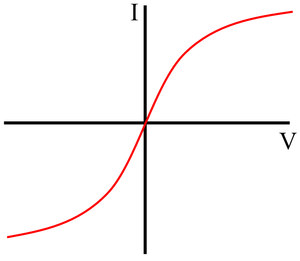
\includegraphics[height=4cm]{Electricity_Images/IV_filament_bulb.png}
    \end{figure}
\end{frame}

\begin{frame}{Diodes}
\begin{multicols}{2}
    Diodes are the electrical equivalent of a one-way street. They let current through in a single direction only, but only after a certain voltage (forward bias) -- however beyond a certain voltage it will break and allow current to flow in reverse (reverse bias). \emph{It is one of few semiconductors that we will see}.
    
    \columnbreak
\begin{figure}
    \centering
    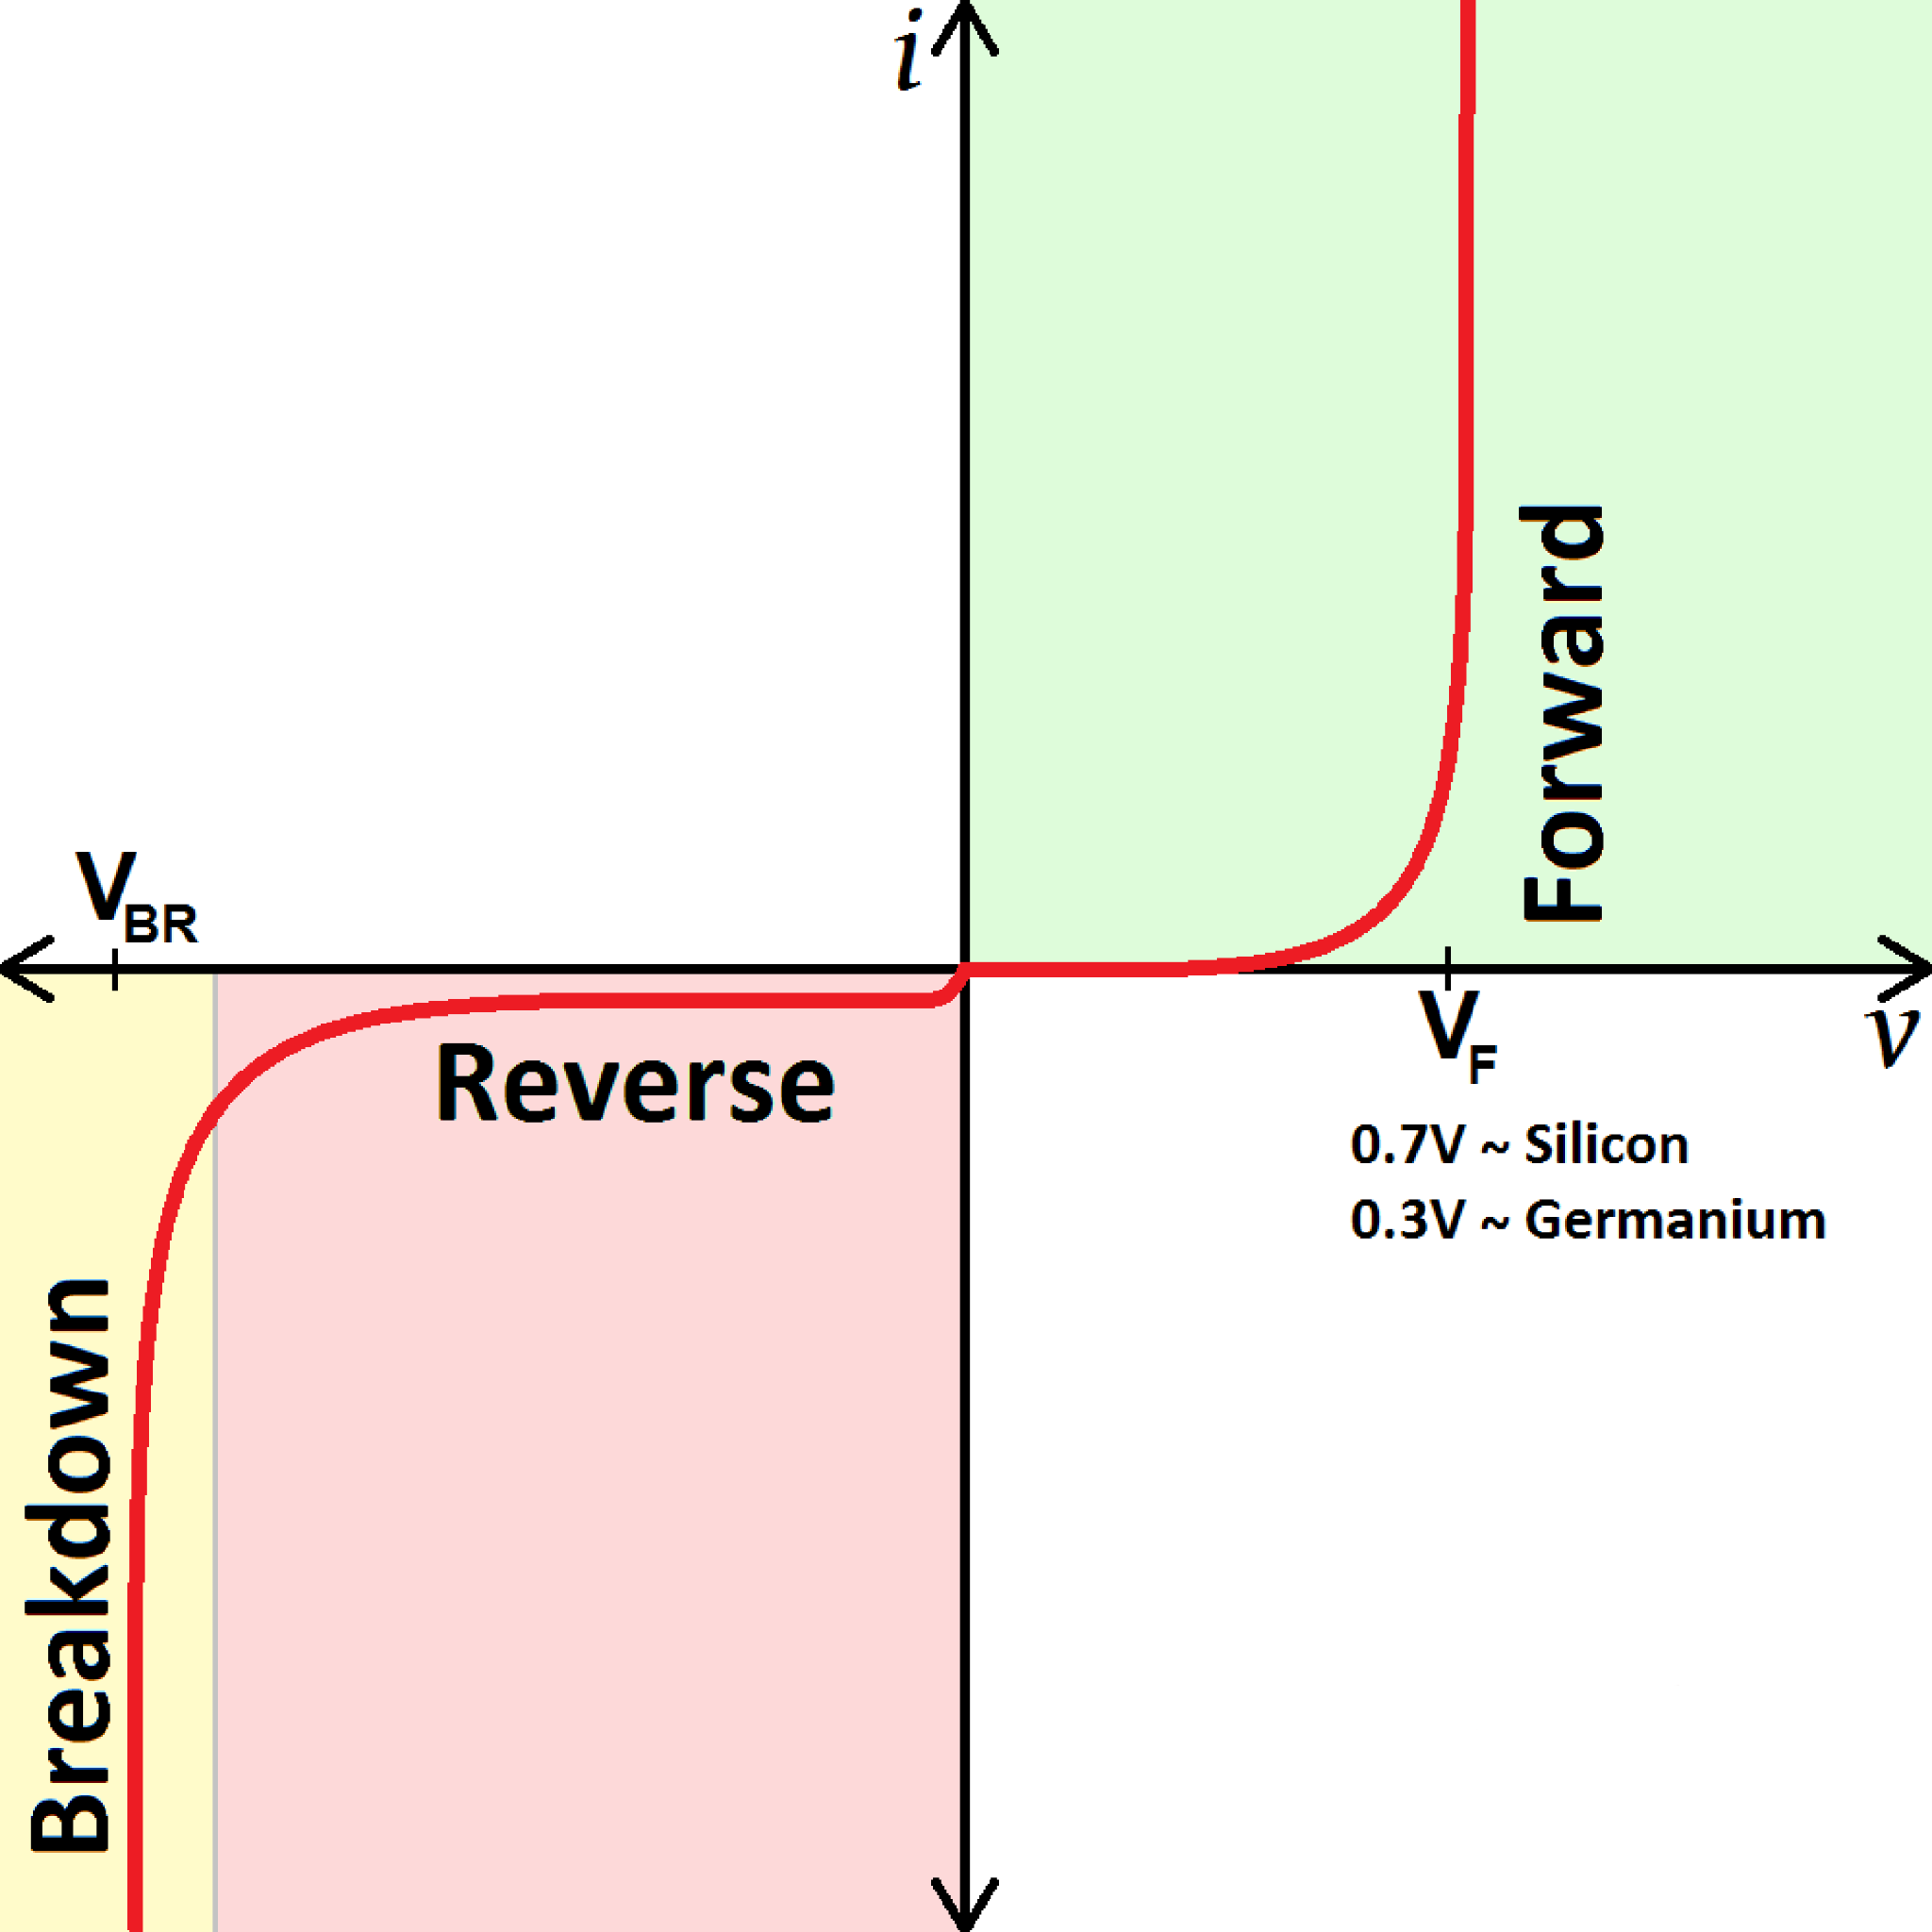
\includegraphics[height=4.5cm]{Electricity_Images/IV_Diode.png}
\end{figure}
\end{multicols}

    \begin{block}{Silicon Diode}
        The diodes we look at are generally silicon-based with a forward bias of 0.7V. There is no general breakdown voltage.
    \end{block}
\end{frame}

\begin{frame}{Diodes}
    
        \begin{figure}
            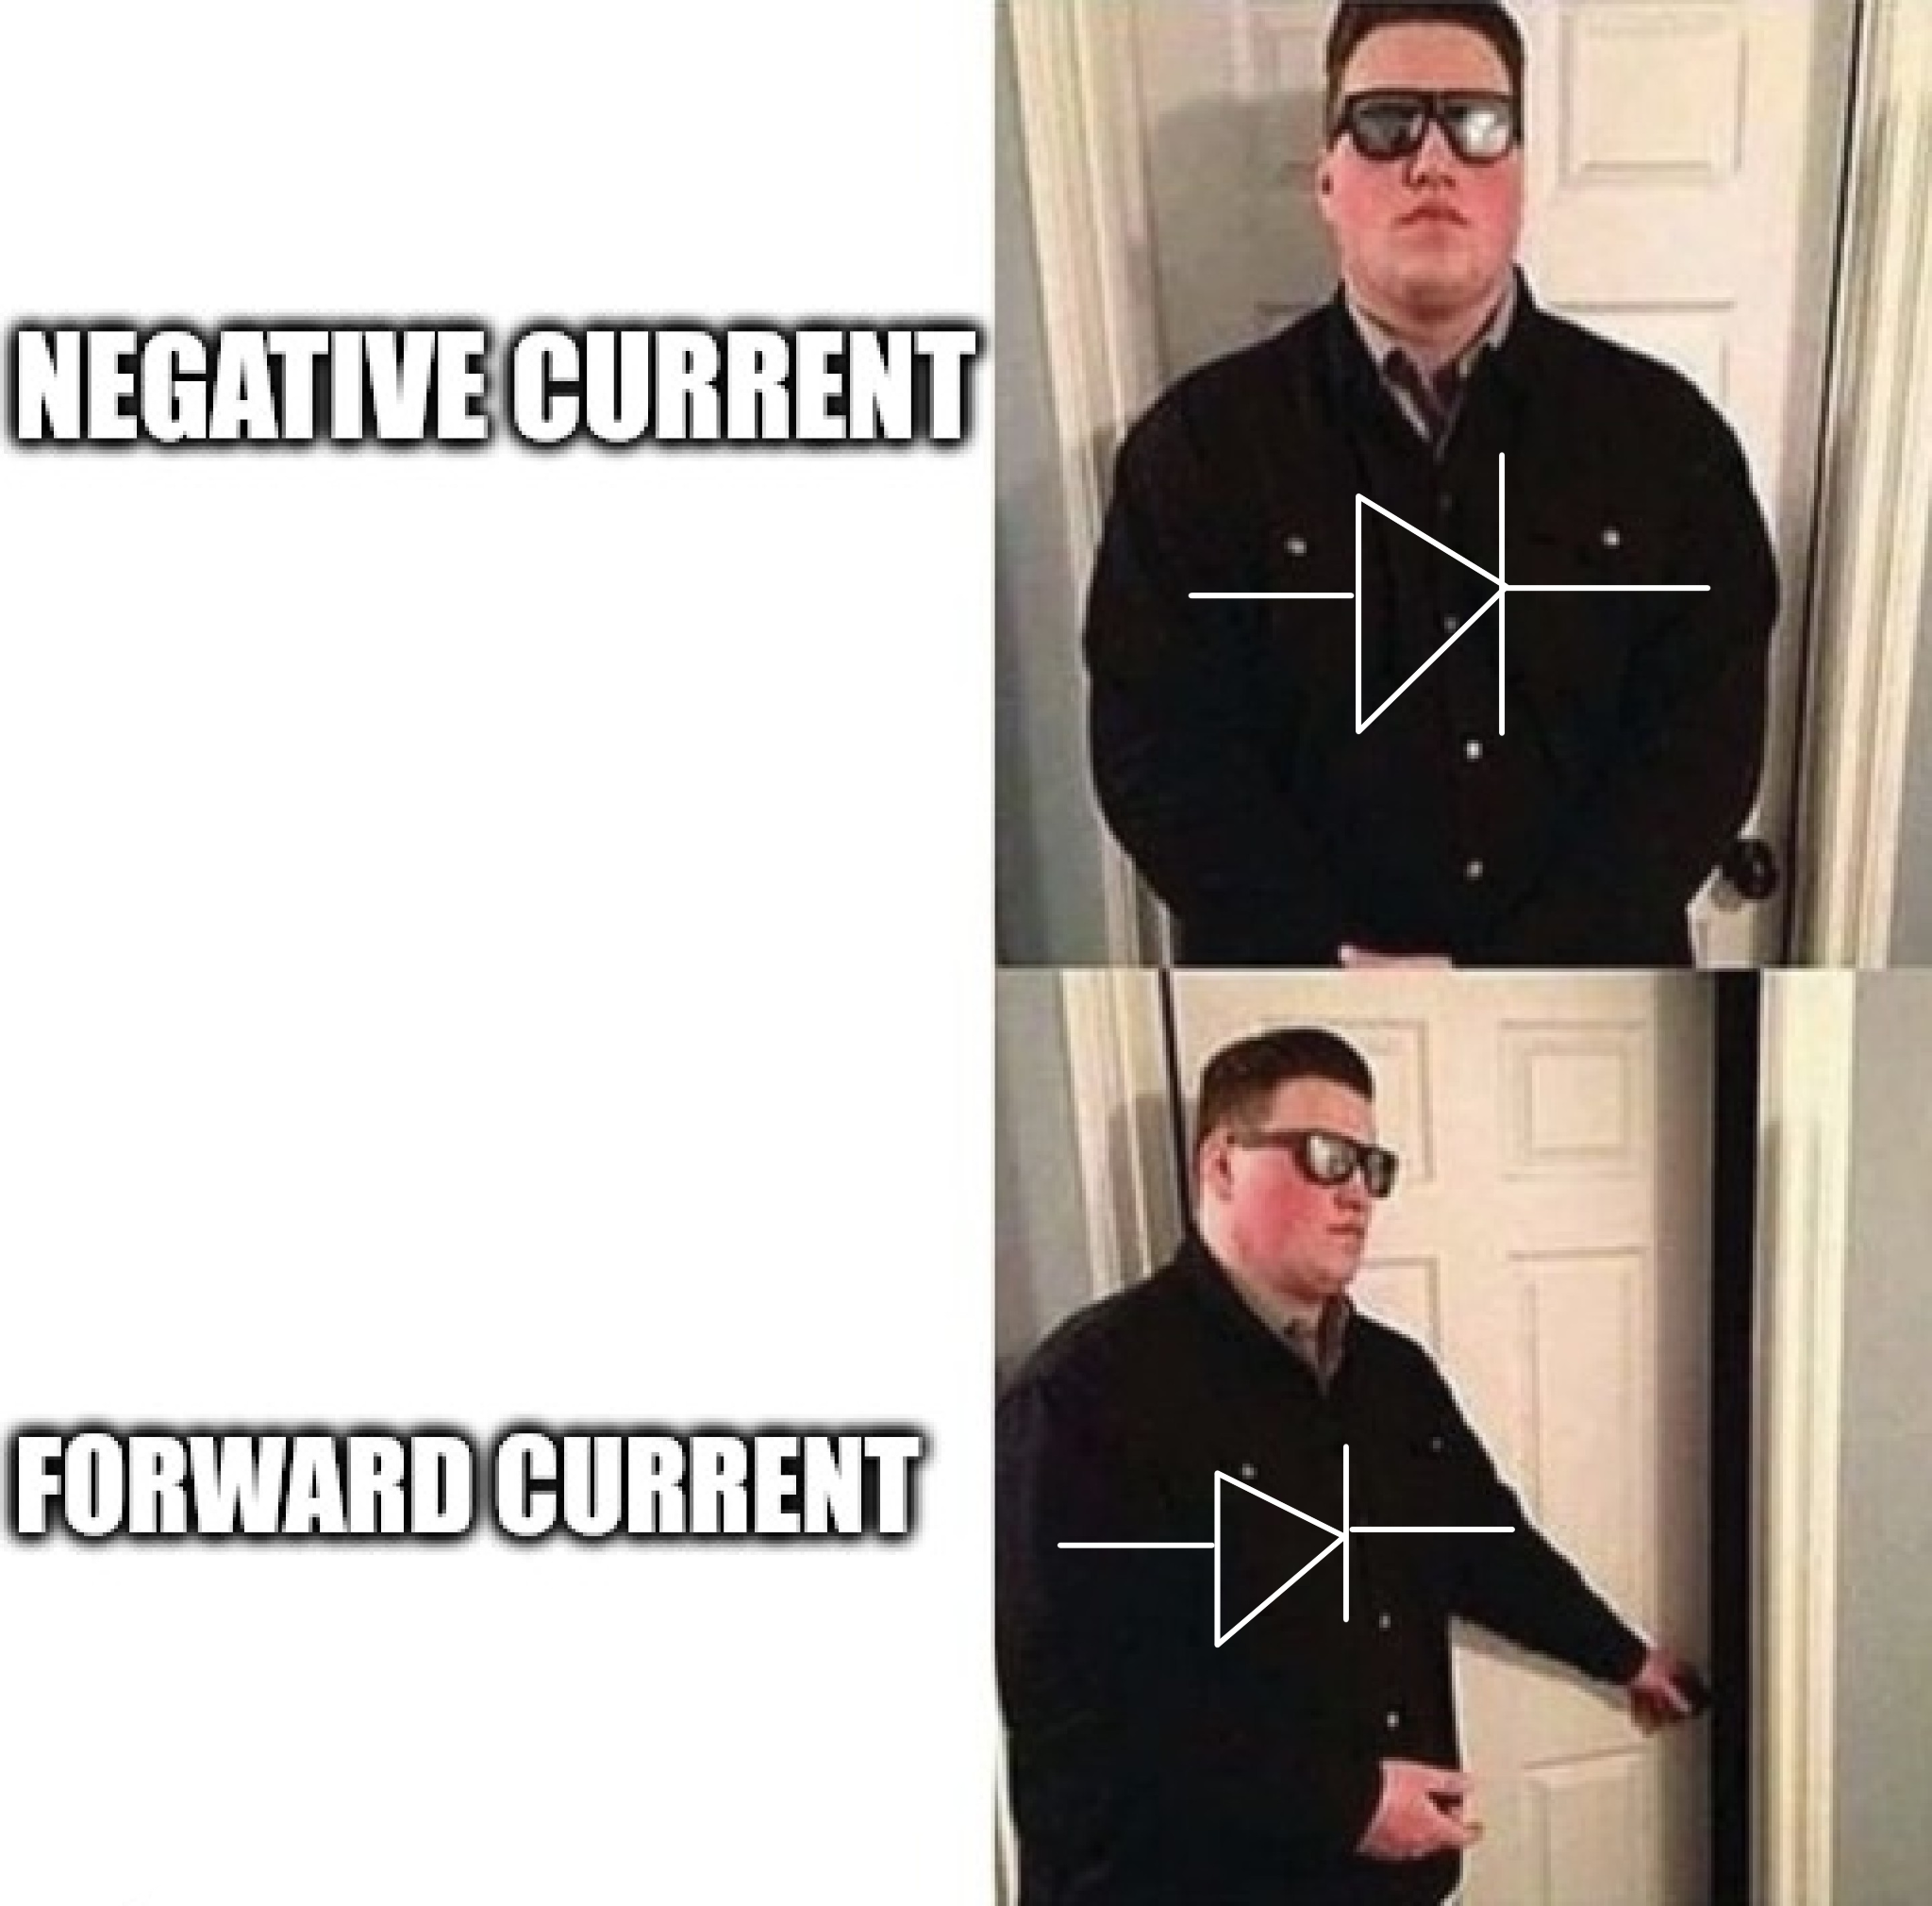
\includegraphics[height=7cm]{Electricity_Images/persuadable_bouncer_diode.png}
            \end{figure}
\end{frame}

\begin{frame}{Diodes in circuits}
If you see a diode in a circuit, know that current can only flow that way -- with the arrow pointing from + to -, or higher p.d to lower. Generally you could be asked about these in multiple choice questions.
\pause
\begin{exampleblock}{Example}
\begin{figure}
    \centering
    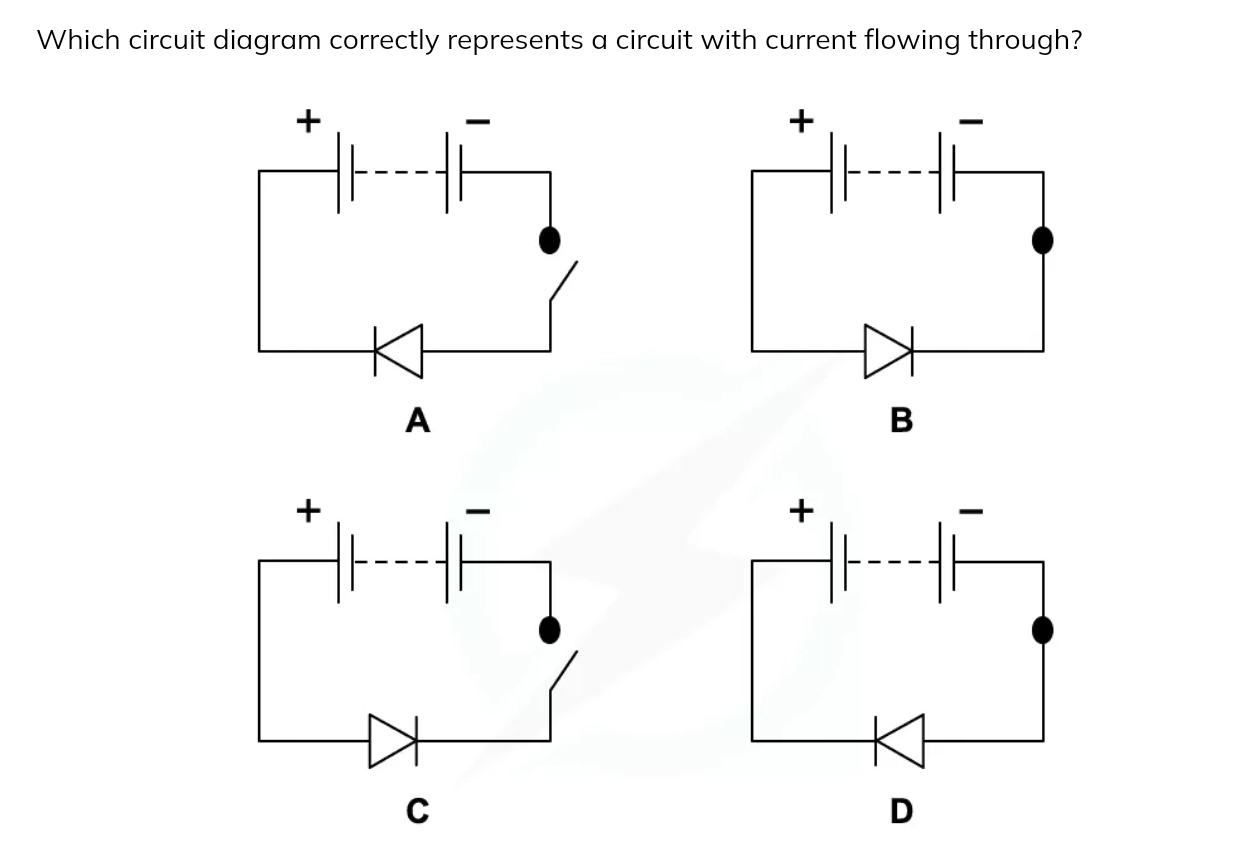
\includegraphics[height=5cm]{Electricity_Images/diodes_mcq.jpg}
\end{figure}
\end{exampleblock}
\end{frame}

\begin{frame}{Thermistors}
    A thermistor changes it's resistance according to the temperature. As such, it does not follow Ohm's law -- the resistance is not constant.
    
    \begin{figure}
        \centering
        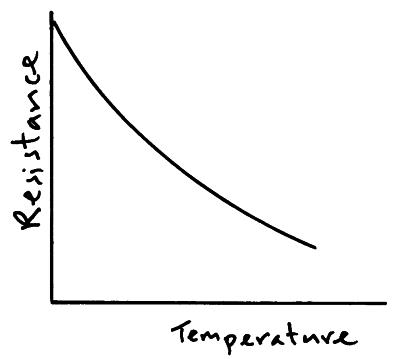
\includegraphics[height=5cm]{Electricity_Images/ntc_thermistor.jpg}
    \end{figure}
    
    A thermistor is said to have a `negative temperature coefficient' (NTC) -- i.e the resistance decreases with increasing temperature.
\end{frame}

\begin{frame}{Temperature Coefficients}
    But it is important to note that thermistors can also have a postive temperature coefficient -- what might this mean? \pause
    \begin{figure}
        \centering
        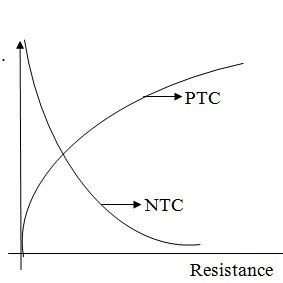
\includegraphics[height=3cm]{Electricity_Images/ptc_thermistor.jpg}
    \end{figure}
    A PTC simply has a resistance that increases with increasing temperature.

    \begin{alertblock}{NTC Thermistors!}
Unless specifically stated you can assume \emph{all} thermistors encounted in exams are NTC. Most questions will be about the application of a thermistor -- what applications could we have?
    \end{alertblock}
\end{frame}

\begin{frame}{Light-dependent resistors}
What do you think a light-dependent resistor might be? \pause
\newline \newline
    A L.D.R. has a similar resistance graph to that of a thermistor, only instead of temperature it is light intensity -- light intensity being the energy transferred by light per second per unit area. $Js^{-1}m^{-2}$ or $Wm^{-2}$.
    
    \begin{figure}
        \centering
        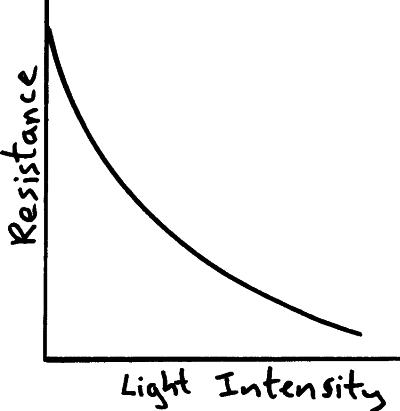
\includegraphics[height=5cm]{Electricity_Images/ldr.jpg}
    \end{figure}
\end{frame}

\end{document}